\title[Alignment of Recordings with Study Materials]{Automatic alignment of Lecture Recordings with Study Materials}
\mode<presentation>{\subtitle[github.com/video699]{\color{black}\faGithub\ \href{https://github.com/video699}{github.com/video699}}}
\author[V.\,Novotný]{Vít Novotný, witiko@mail.muni.cz}
\year=2018\month=11\day=26
\institute[FI MU]{Faculty of Informatics, Masaryk University}
\subject{Research project report}
\keywords{information retrieval, image processing, pattern recognition, machine learning}

\begin{document}
\begin{frame}[plain]
\maketitle
\begin{tikzpicture}[overlay,remember picture]
    \node[anchor=south east, xshift=-38pt, yshift=20pt] at (current page.south east) {
      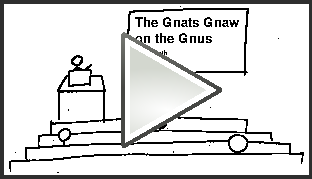
\includegraphics[width=70mm]{figs/gnus-gnats/recording}
    };
\end{tikzpicture}
\end{frame}

% \begin{frame}{Contents}
% \begin{multicols}{2}
% \tableofcontents
% \end{multicols}
% \end{frame}

\section{Introduction}

\begin{frame}{Introduction \smash{\cite[sec.~1]{novotny18}}}
\begin{itemize}
\item<1-7> \abbr{FI} \abbr{MU} has been \alert{recording lectures} and publishing the
  recordings since 2014~\cite{hladkaliska03lectures}.
\item<3-7> Two years of knowledge are archived with \alert{no indexing} and
  \alert{no metadata}.
\item<4-7> \abbr{SPEECH@FIT} use \alert{speech recognition} to annotate videos at
  \href{https://superlectures.com/}{superlectures.com}.
\item<5-7> We use \alert{digital image processing} to map recordings to lecture
  materials.
\item<7> We published our system, and datasets under \alert{open licenses}
  at \href{https://github.com/video699}{github.com/video699}.
\end{itemize}

\begin{center}
\only<1>{\vspace{-2cm}\includegraphics[height=0.7\textheight]{figs/gnus-gnats/lecture-01}}
\only<2>{\vspace{-3.5cm}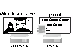
\includegraphics[height=0.82\textheight]{figs/gnus-gnats/storage}}
\only<3>{\vspace{-1.8cm}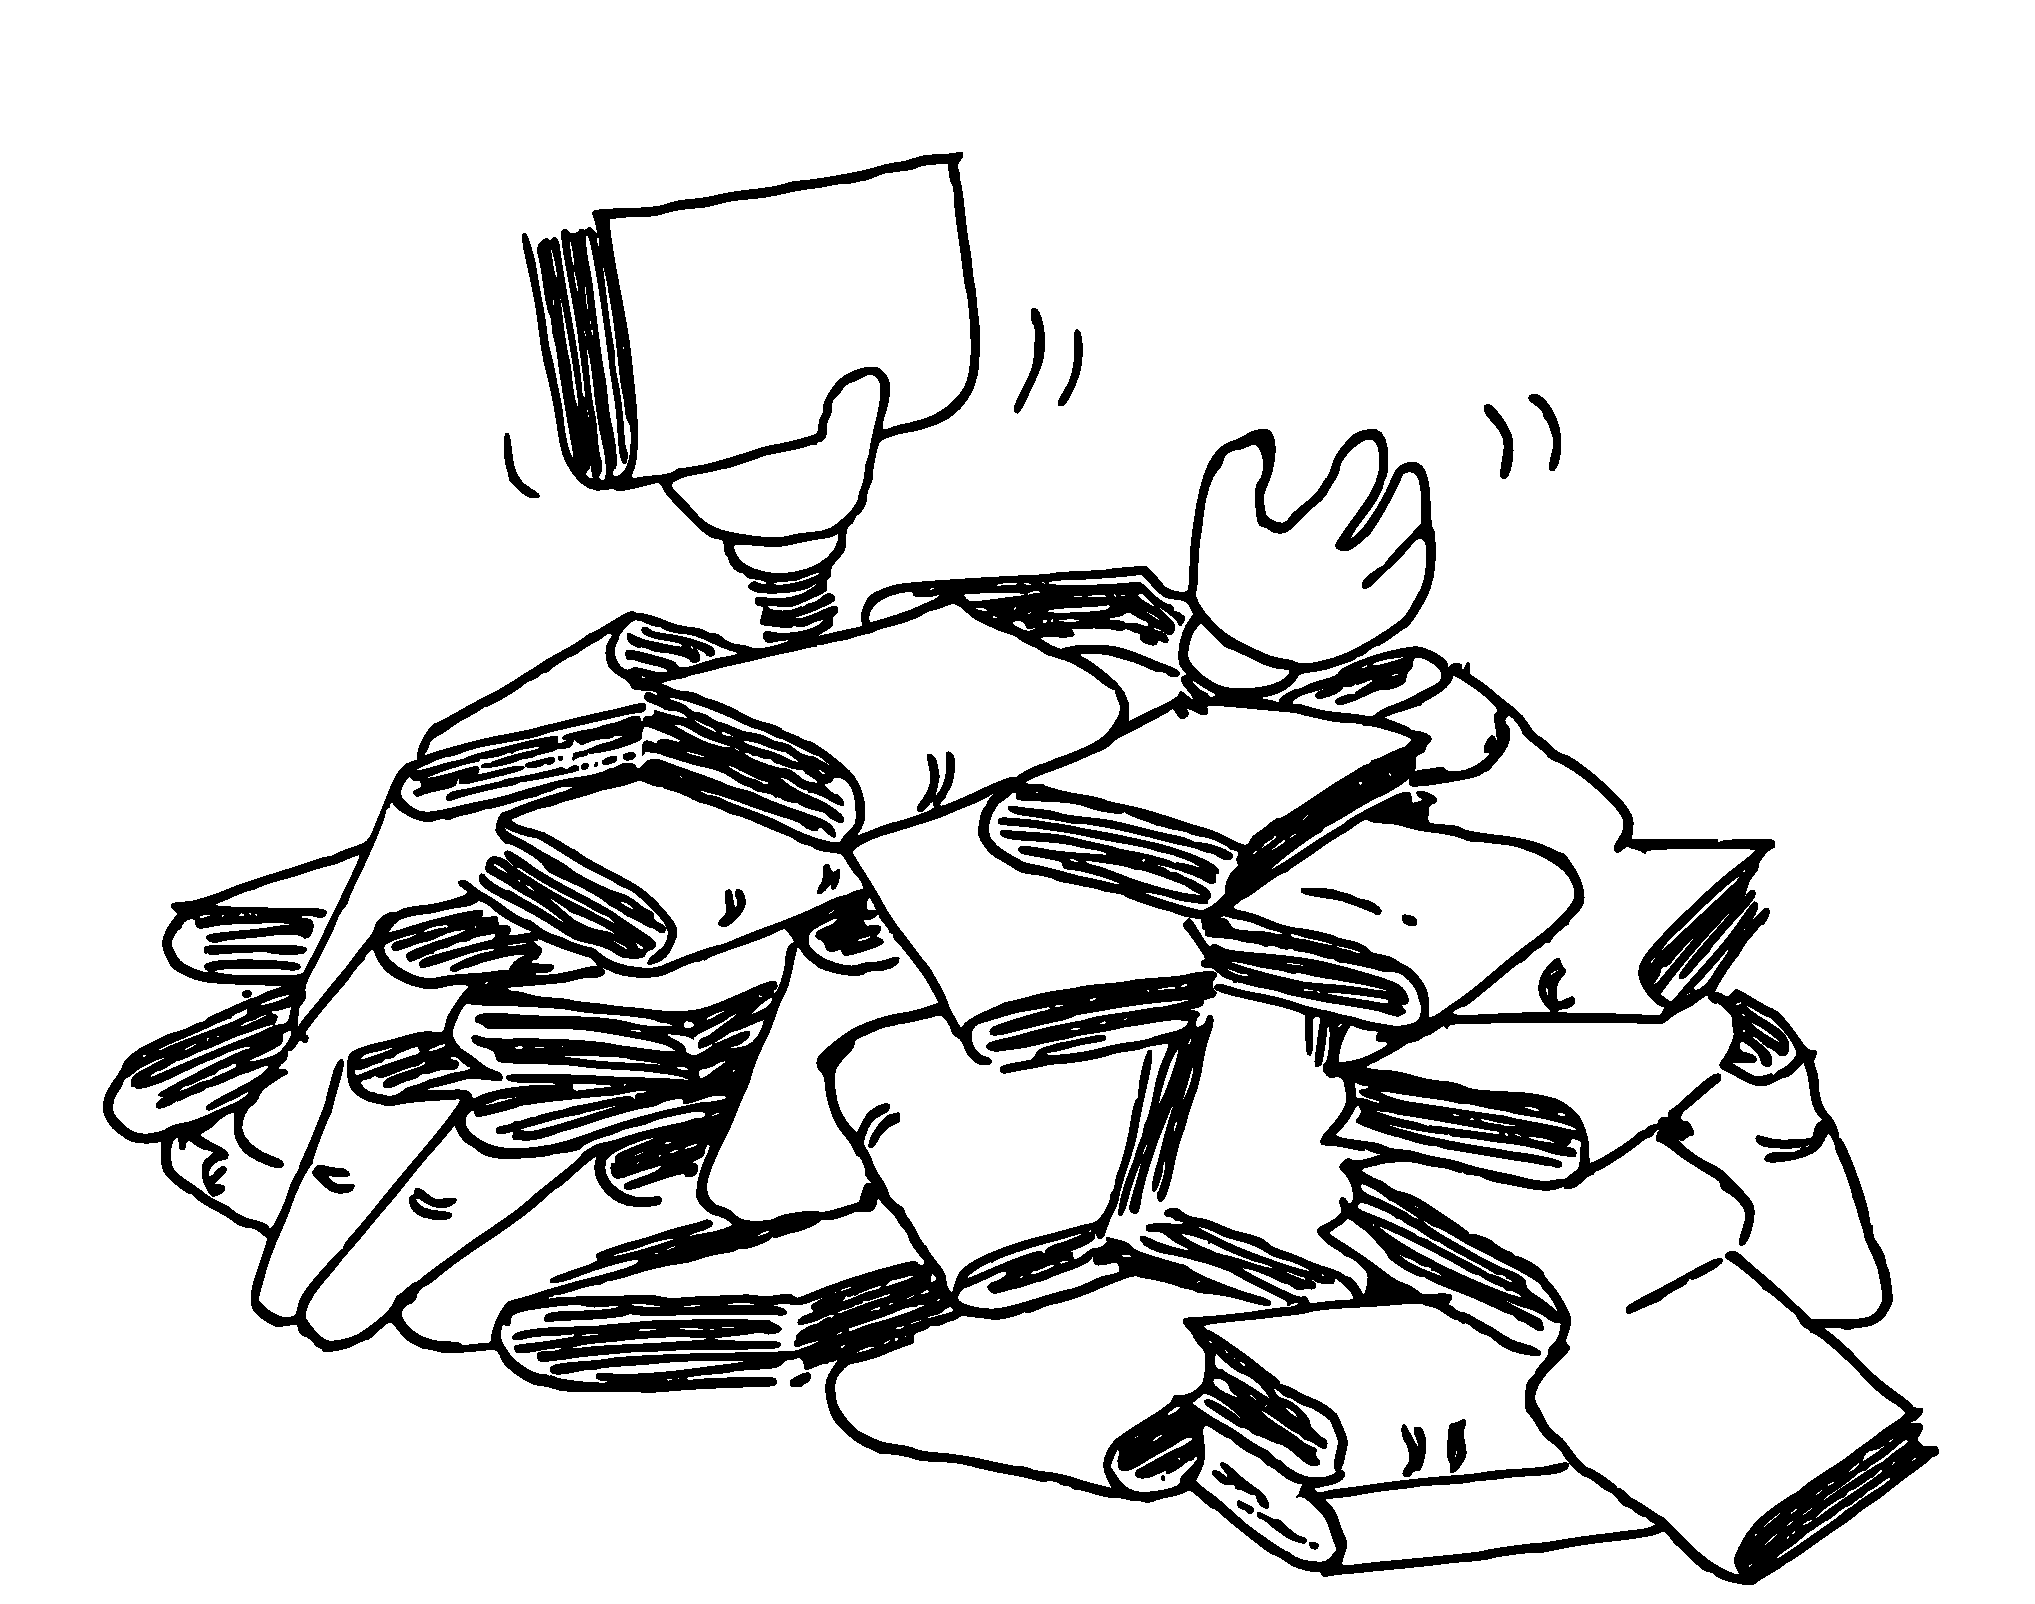
\includegraphics[height=0.65\textheight]{figs/franek/overload}}
\only<4>{\vspace{-1.8cm}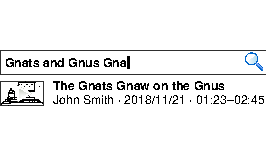
\includegraphics[height=0.7\textheight]{figs/gnus-gnats/search-results}}
\only<5>{\vspace{-1cm}\includegraphics[height=0.6\textheight]{figs/gnus-gnats/mapping}}
\only<6>{\vspace{-1.8cm}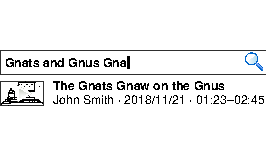
\includegraphics[height=0.7\textheight]{figs/gnus-gnats/search-results}}
\only<7>{%
  
\includegraphics[height=0.4\textheight]{figs/logo/gplv3}%
  \hspace{1cm}
  
\includegraphics[height=0.4\textheight]{figs/logo/ok}%
}
\end{center}

\end{frame}

\section{Tasks}

\begin{frame}{Tasks \smash{\cite[sec.~2.2]{novotny18}}}
\begin{itemize}
\item<1-5> Given a set of \alert{lecture materials}, and a set of \alert{lecture
  recordings}, we need to produce a set of \alert{time segments} during which a
  recording displays a lecture material.
\item<2-5> We break this high-level task into \alert{four elementary subtasks}:
\begin{description}
\item<2-5>[FRAMES] Detect \alert{significant video frames}, where lecture
  materials transition.
\item<3-5>[SCREENS] Detect \alert{projection screens} in a significant video
  frame.
\item<4-5>[RETRIEVAL] Find the \alert{nearest lecture materials} to a projection
  screen.
\item<5-5>[MATCHING] Decide if any nearest lecture materials \alert{matches}
  the projection screen.
\end{description}
\end{itemize}

\begin{center}
\only<1>{\vspace{-3cm}\includegraphics[height=0.7\textheight]{figs/gnus-gnats/mapping}}%
\only<2>{\vspace{-1.5cm}\hspace{3cm}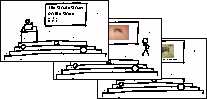
\includegraphics[height=0.53\textheight]{figs/gnus-gnats/frames}}%
\only<3>{\vspace{-1.9cm}
\includegraphics[height=0.6\textheight]{figs/gnus-gnats/screens}}%
\only<4>{\vspace{-1.9cm}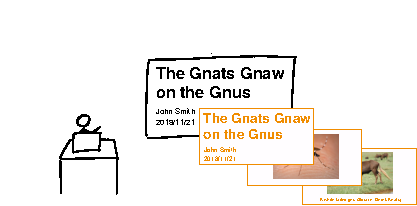
\includegraphics[height=0.6\textheight]{figs/gnus-gnats/retrieval}}%
\only<5>{\vspace{-0.1cm}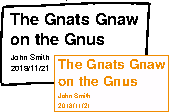
\includegraphics[height=0.3\textheight]{figs/gnus-gnats/matching}}%
\end{center}
\end{frame}

\section{Datasets}

\begin{frame}{Datasets \smash{\cite[sec.~3]{novotny18}}}
\begin{itemize}
\item<1-11> We need a dataset~\cite{implementation-dataset} for
  \alert{supervised learning} to \alert{evaluate} our system:
\begin{itemize}
\item<1-11> We collected a random sample of \alert{17 lecture recordings} from 2010--2016.
\item<2-11> We drew a stratified sample of \alert{up to 25 video frames} from each recording.
\item<4-11> In each frame, we annotated \alert{lit projection screens} and
  their condition.
\item<6-11> For each lit projection screen, we annotated \alert{lecture materials} shown in
  the screen.
\item<8-11> The dataset contains \alert{699 projection screen annotations}, and
  \alert{925 lecture materials}.
\end{itemize}
\item<9-11> We need a dataset~\cite{implementation-screens} to solve
  \task{SCREENS}:
\begin{itemize}
\item<9-11> We annotated \alert{three rooms} at \abbr{FI MU}.
\item<10-11> In each room, we anotated \alert{camcoders}, and \alert{projection screens}.
\item<11-11> We annotated \alert{positions of screens} in the coordinates of
  every camcoder across time.
\end{itemize}
\end{itemize}

\begin{center}
\only<1,2,4,6,8-11>{%
  \vspace{-2cm}
  \only<1>{%
    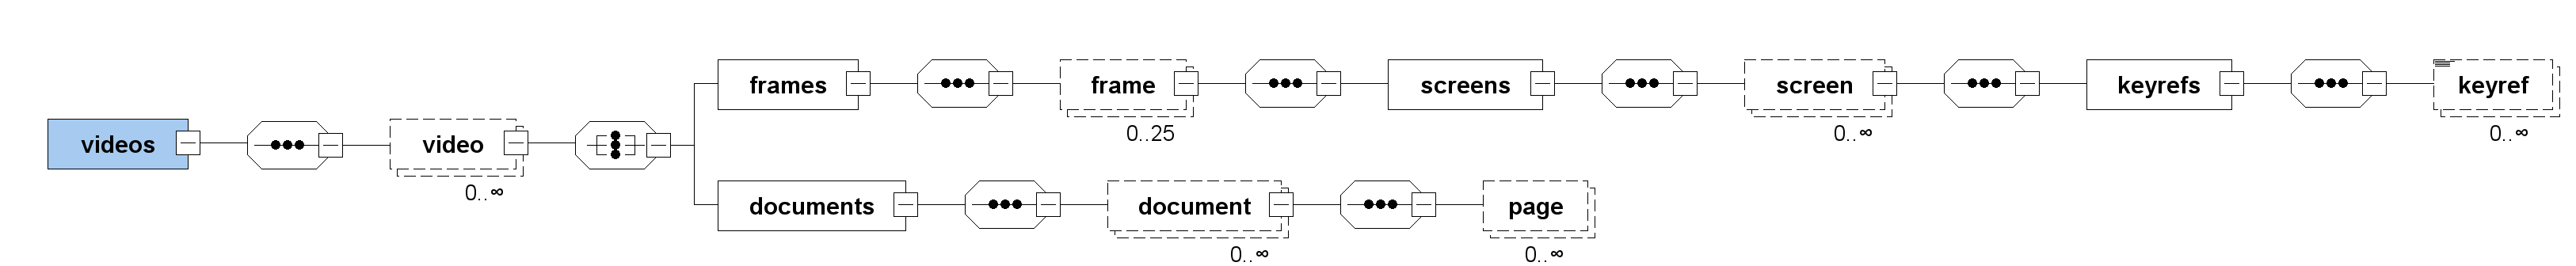
\includegraphics[width=2\textwidth]{figs/diagram/implementation-dataset_videos}%
  }%
  \only<2>{%
    \hspace*{-3cm}%
    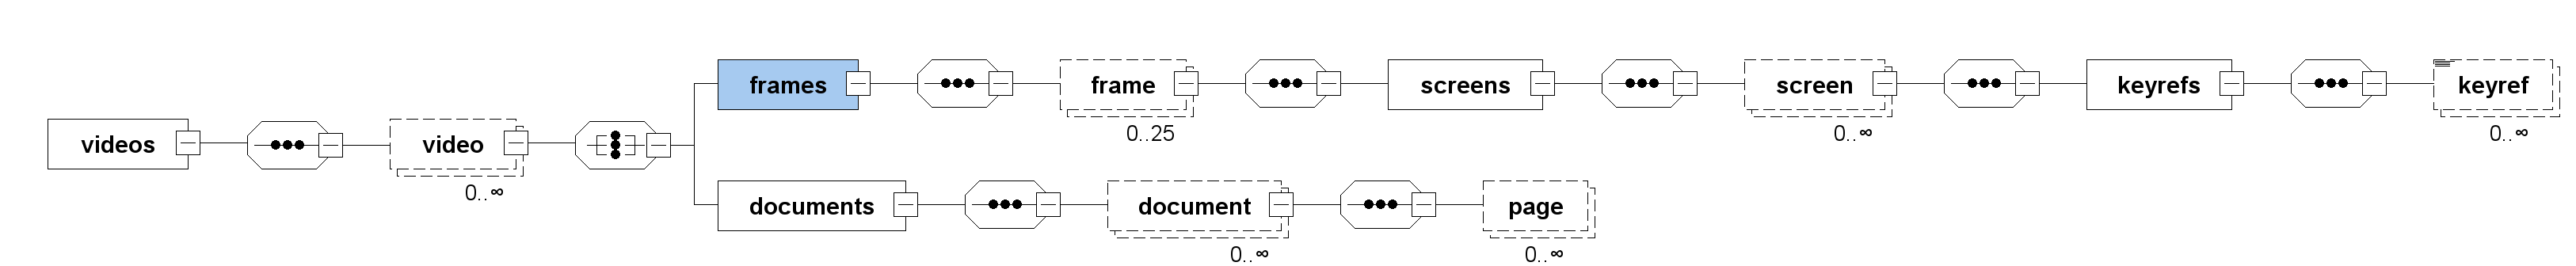
\includegraphics[width=2\textwidth]{figs/diagram/implementation-dataset_frames}%
  }%
  \only<4>{%
    \hspace*{-6.5cm}%
    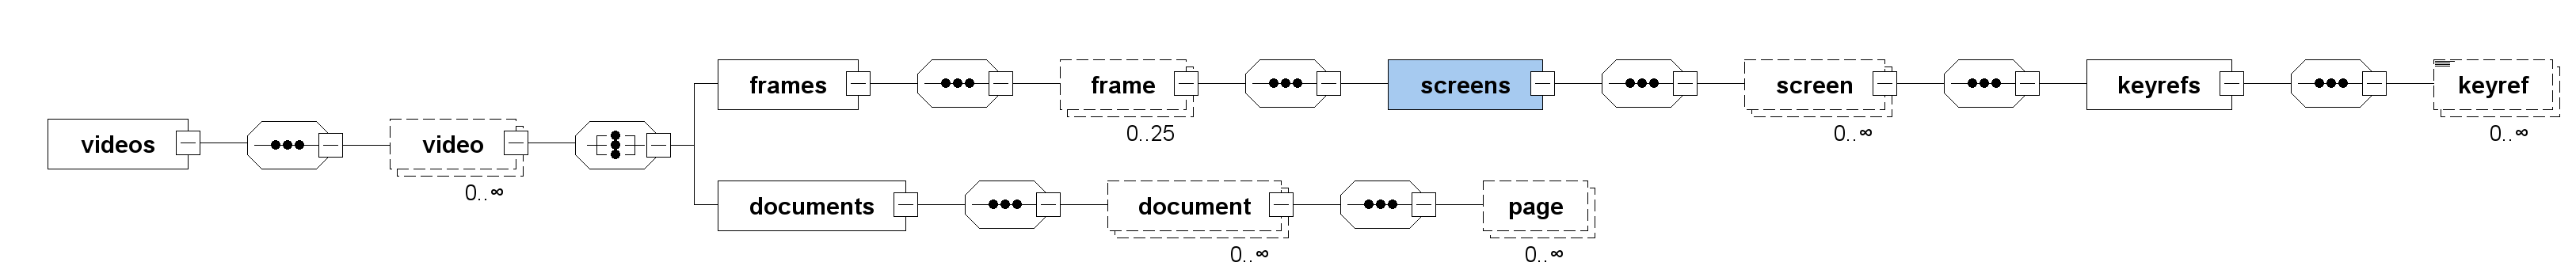
\includegraphics[width=2\textwidth]{figs/diagram/implementation-dataset_screens}%
  }%
  \only<6>{%
    \hspace*{-14cm}%
    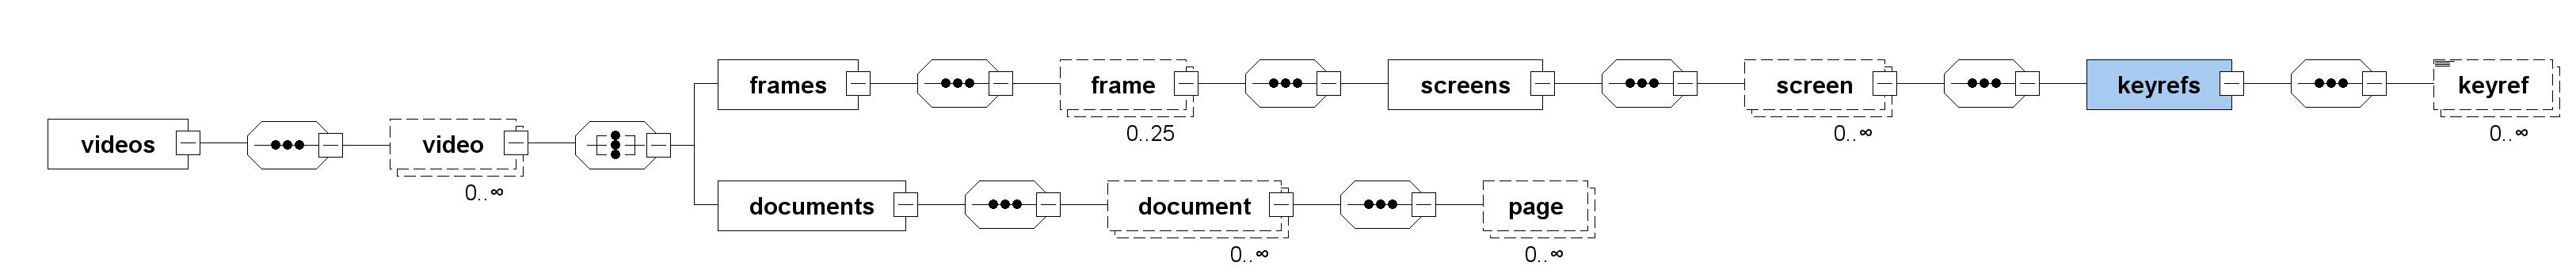
\includegraphics[width=2\textwidth]{figs/diagram/implementation-dataset_keyrefs}%
  }%
  \only<8>{%
    \vspace{0.35cm}
    \hspace*{-15cm}%
    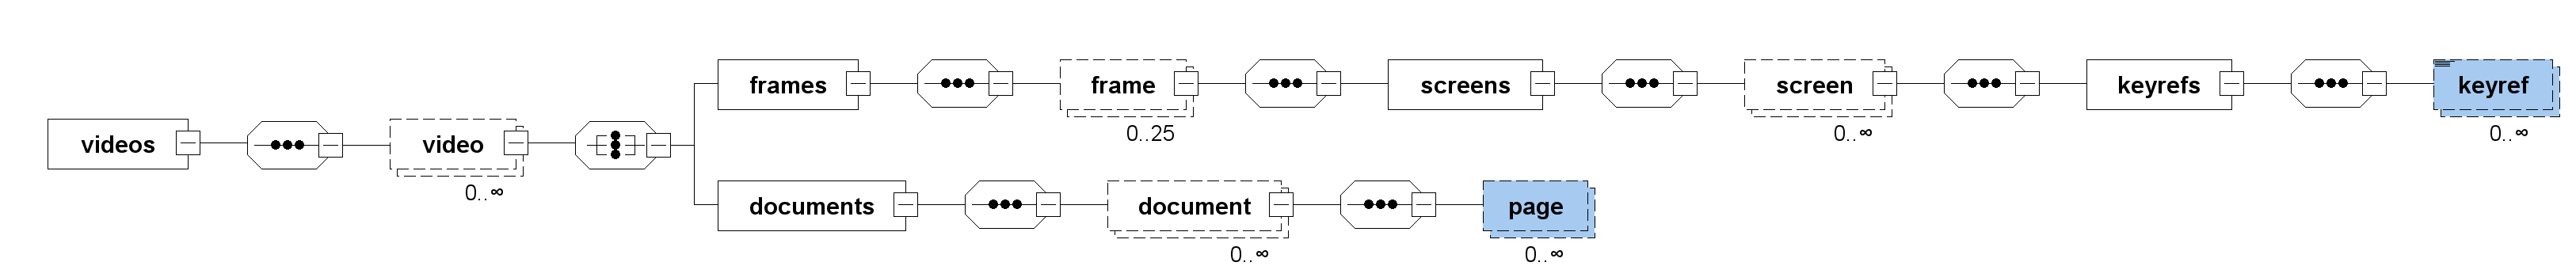
\includegraphics[width=2\textwidth]{figs/diagram/implementation-dataset_keyref_page}%
  }%
  \only<9>{%
    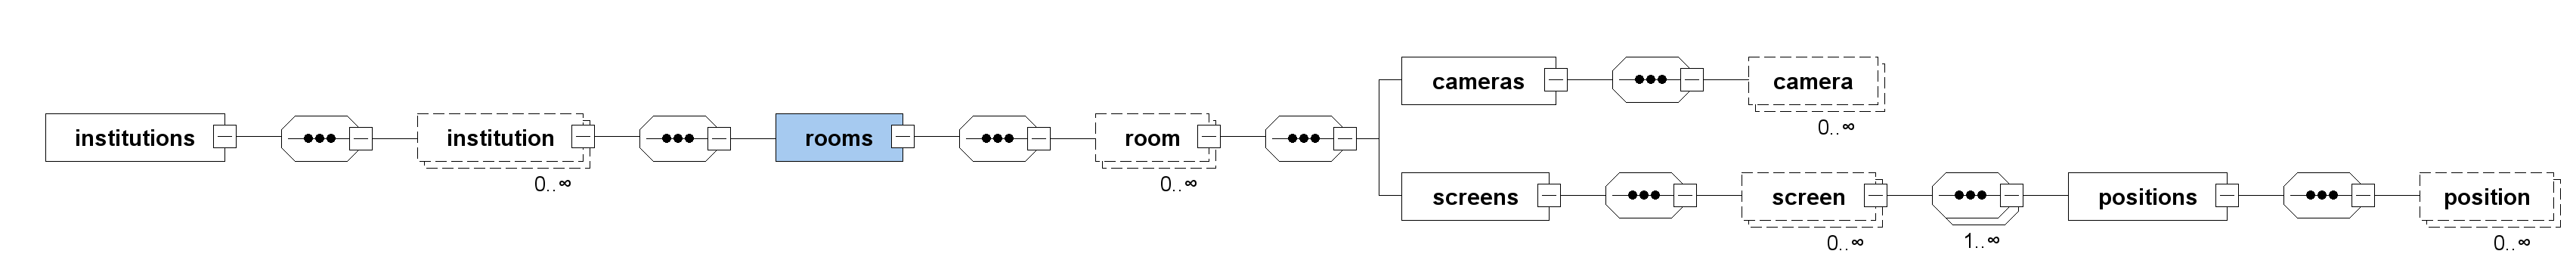
\includegraphics[width=2\textwidth]{figs/diagram/implementation-screens_rooms}%
  }%
  \only<10>{%
    \hspace*{-3cm}%
    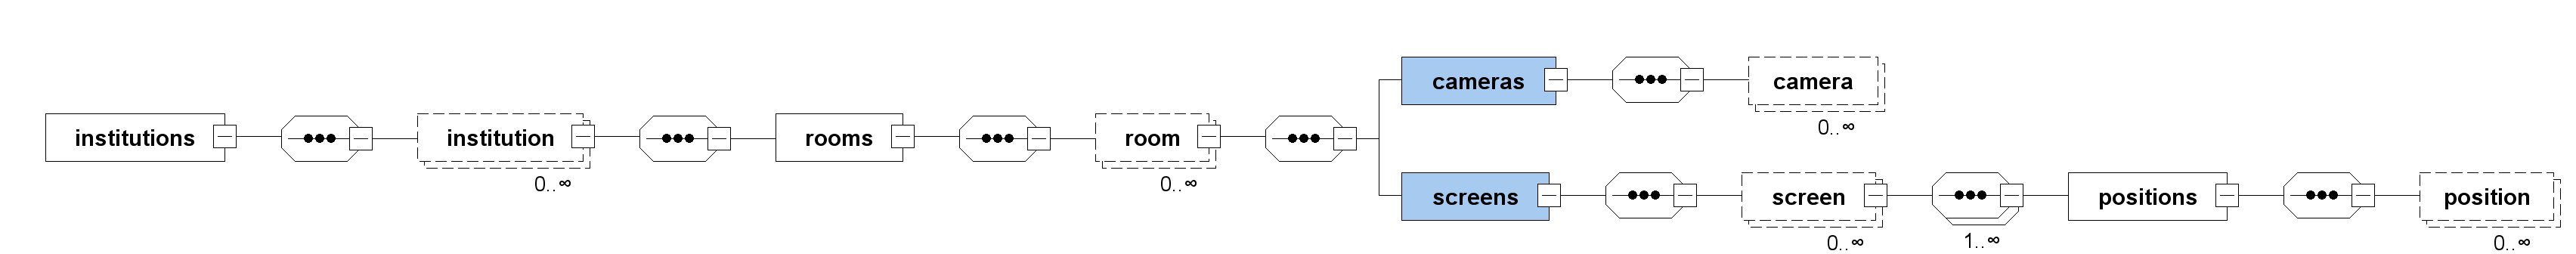
\includegraphics[width=2\textwidth]{figs/diagram/implementation-screens_camcoders_screens}%
  }%
  \only<11>{%
    \hspace*{-14.5cm}%
    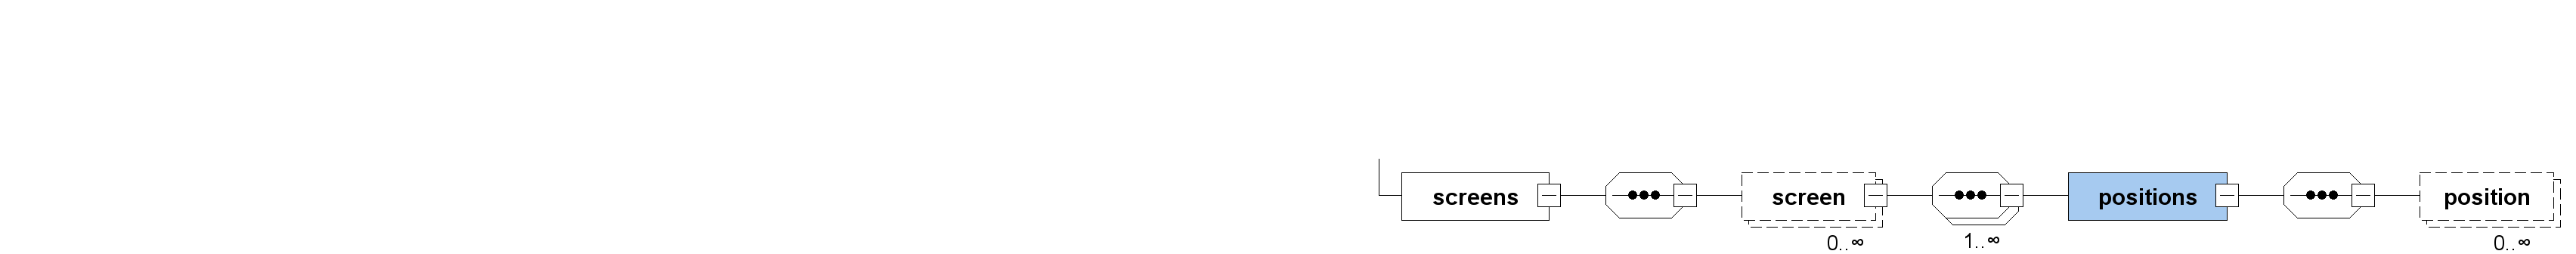
\includegraphics[width=2\textwidth]{figs/diagram/implementation-screens_positions}%
  }%
}%
\only<3>{%
  \vspace{-2cm}\leavevmode
  \includegraphics[width=0.3\textwidth]{implementation-videos/PA152-D3-20110331.avi/frame002000}
  \includegraphics[width=0.3\textwidth]{implementation-videos/PA152-D3-20110331.avi/frame004000}
  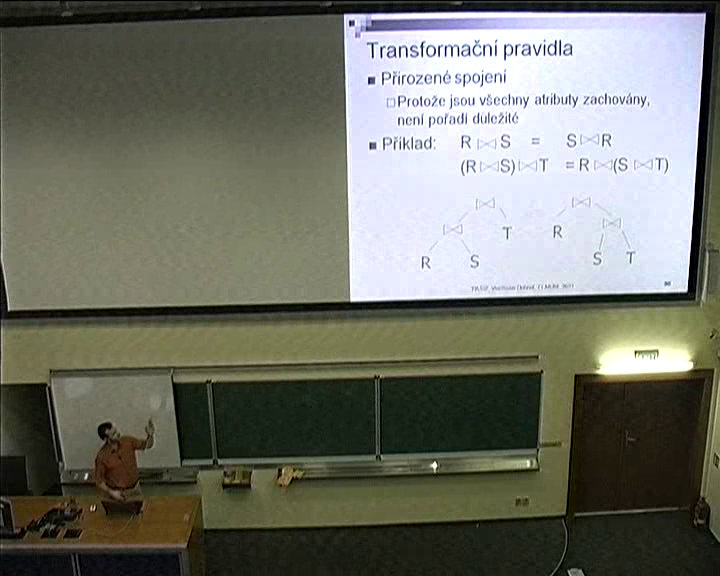
\includegraphics[width=0.3\textwidth]{implementation-videos/PA152-D3-20110331.avi/frame006000}%
}%
\only<5>{%
  \vspace{-2.2cm}\leavevmode
  \includegraphics[align=c, width=0.3\textwidth]{figs/dataset-examples/beyond-bounds/frame004000}
  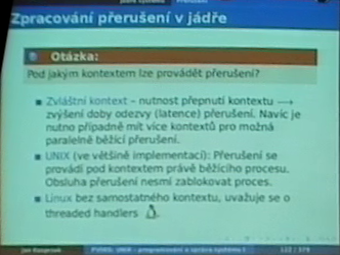
\includegraphics[align=c, width=0.3\textwidth]{figs/dataset-examples/beyond-bounds/frame004000-00}
  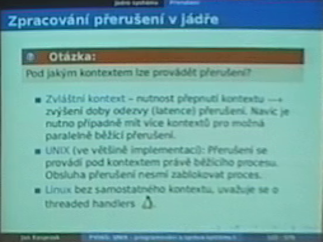
\includegraphics[align=c, width=0.3\textwidth]{figs/dataset-examples/beyond-bounds/frame004000-01}%
}%
\only<7>{%
  \vspace{-2cm}\leavevmode
  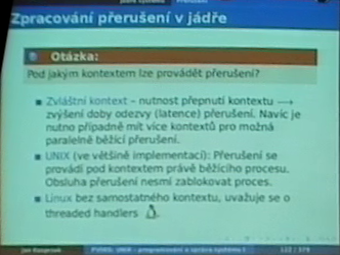
\includegraphics[width=0.3\textwidth]{figs/dataset-examples/beyond-bounds/frame004000-00}
  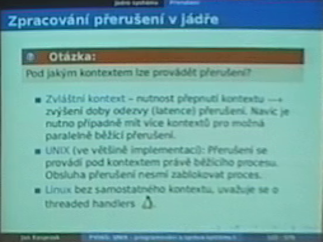
\includegraphics[width=0.3\textwidth]{figs/dataset-examples/beyond-bounds/frame004000-01}
  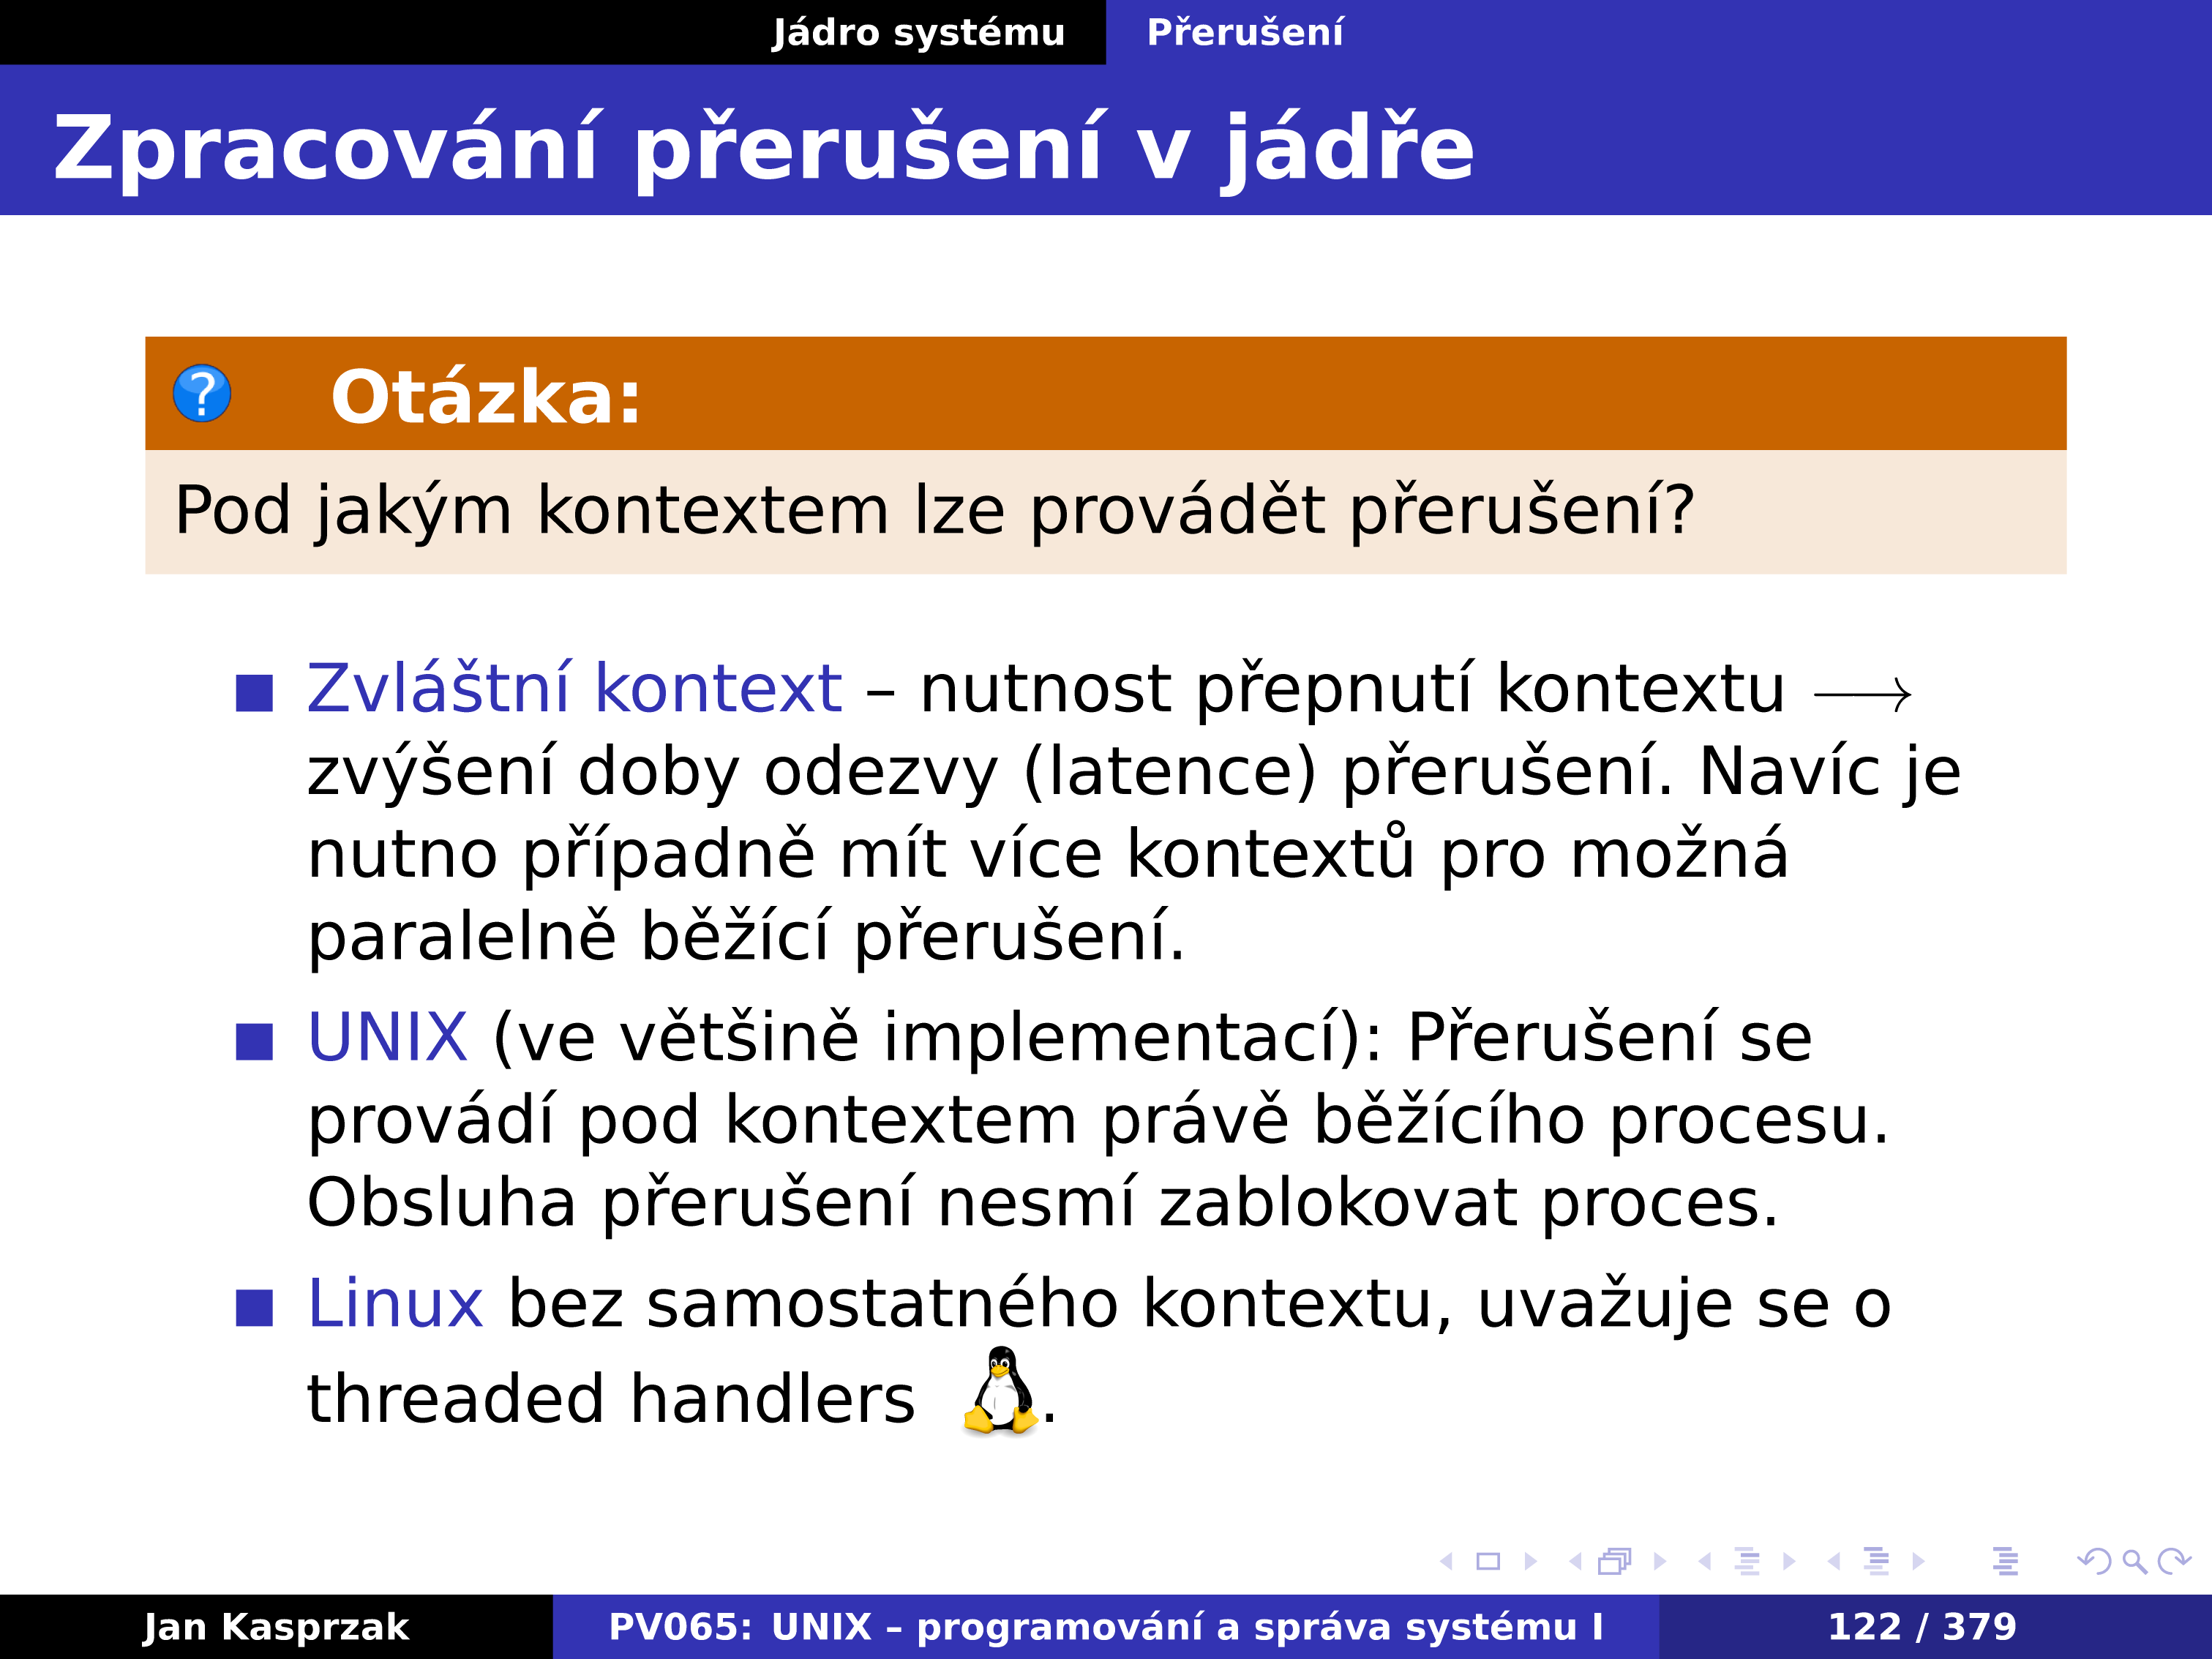
\includegraphics[width=0.3\textwidth]{figs/dataset-examples/beyond-bounds/slides01-12}%
}%
\end{center}
\end{frame}

\section{System}
\section{Evaluation}
\section{Results}
\section{Conclusion}
\section{Future Work}
\section{Acknowledgements}

\section{Bibliography}

\begin{frame}[allowframebreaks]{Bibliography}
\printbibliography
\end{frame}
\end{document}
